%!TeX spellcheck = en-GB

%Basics
\documentclass[aps, prb, a4paper, english, 12pt, onecolumn, longbibliography, amsmath, amssymb, colorinlistoftodos, floatfix]{revtex4-1}
\usepackage[utf8]{inputenc}
\usepackage{babel}

%Symbols and scientifics
\usepackage{amsmath, amsfonts, amssymb, bm}
\usepackage{physics}
\usepackage{mathtools}
\usepackage{siunitx}
\sisetup{
	per-mode = power ,
	round-mode = figures ,
	round-precision = 3 ,
	scientific-notation = false ,
	output-decimal-marker = {.} ,
	exponent-product = \times ,
	separate-uncertainty = true ,
	uncertainty-separator = \ ,
	output-product = \cdot ,
	quotient-mode = fraction ,
	range-phrase = - ,
	range-units =  single ,
	inter-unit-product = \ensuremath{{\cdot{}}} ,
	number-unit-product = \ ,
	multi-part-units = single ,
	alsoload = synchem ,
	alsoload = addn
}
\DeclareSIUnit\atm{atm}

%Appendix, TOC and Bibliography
\usepackage{appendix}
\renewcommand\appendixtocname{Appendices}
%\usepackage[nottoc]{tocbibind}
\usepackage[lastpage,user]{zref}

%Figures
\usepackage[svgnames]{xcolor} % Required to specify font color
\usepackage{float}
\usepackage{graphicx}
\usepackage{subcaption}
\usepackage[format=plain,
            labelfont={bf,it},
            textfont=it]{caption}
\usepackage[verbose]{wrapfig}
\usepackage[a4paper, centering, rmargin=2.5cm, tmargin=2.5cm, lmargin=2.5cm, bmargin=2.5cm]{geometry}
\usepackage{etoolbox}
\usepackage{verbatim}
\usepackage[space]{grffile}
\usepackage[final]{pdfpages}
\usepackage{array}
\usepackage{multirow}
\usepackage{dcolumn}
%\usepackage{animate}
\usepackage{fontawesome}
\usepackage[european]{circuitikz}
\usepackage{pgfplots}
\pgfplotsset{width=10cm}
\def\axisdefaultwidth{10cm}
%\usepgfplotslibrary{external}
\usepgfplotslibrary{units}
%\tikzexternalize

%Header footer
\usepackage{fancyhdr}
\pagestyle{fancy}
\lhead{N. Kihm \\ R. K. F. Wiuff}
\chead{Course 10401\\Fusion Energy and Plasma Physics}
\rhead{January \nth{24}\\2019}
\cfoot{Page \thepage\, of \zpageref{LastPage}}
\renewcommand{\headrulewidth}{0.4pt}
\renewcommand{\footrulewidth}{0.4pt}

%Text tools
\usepackage[super]{nth}
\usepackage[normalem]{ulem}
\usepackage{import}
\usepackage{url}
\usepackage{lipsum}
\usepackage{microtype}
\usepackage[pdfencoding=auto, psdextra]{hyperref}
\hypersetup{
	colorlinks   = true, %Colours links instead of ugly boxes
	urlcolor     = blue, %Colour for external hyperlinks
	linkcolor    = blue, %Colour of internal links
	citecolor   = red %Colour of citations
}
\usepackage[capitalise]{cleveref}
\usepackage{enumitem}
\setlist[enumerate]{itemsep=0mm}
\usepackage{booktabs}
\usepackage{silence}
\usepackage{todonotes}
\WarningFilter{revtex4-1}{Repair the float}

%Python
\usepackage{minted}
\setminted{fontsize=\small}
\usemintedstyle{monokai}
\renewcommand{\listoflistingscaption}{Listings}
%\renewcommand{\MintedPygmentize}{C:/Users/rwiuf/AppData/Roaming/Python/Python37/Scripts/pygmentize}

%Definitions and new commands
\newcommand{\degr}{^{\circ}}
\newcommand{\me}{\mathrm{e}}
\newcommand*\mathinhead[2]{\texorpdfstring{$\boldsymbol{#1}$}{#2}}
%PDFPages and RevTeX incompatability fix
\makeatletter
\AtBeginDocument{\let\LS@rot\@undefined}
\makeatother

\begin{document}
%Titlepage herunder:
\begin{abstract}
	\vspace{5mm}
	\centering
	\includegraphics[width=.5\textwidth]{Figures/ITERmachine.jpg}
	\begin{description}
		\item[Abstract] Plasma fusion for energy production is a growing scientific field with interests all over the globe as clean and sustainable energy as well as growing energy demands needs to be addressed. In the course ``10401: Fusion energy and plasma physics'' we deal with some of the fundamental engineering aspects of a commercial fusion energy power plant, as well as the research towards this goal. In this paper we first address a simple model for such a plant and how the model can be improved upon. Secondly we investigate how to diagnose plasma density with simple interferometry in the DTU tokamak reactor. Lastly we made measurements in the DTU fusor, and investigated some energy production aspects with such a device. \vspace{3\baselineskip}
	\end{description}
	\includegraphics[width=1cm]{Figures/DTU3CMYK.eps}
\end{abstract}

\title{10401\\Fusion Energy and Plasma Physics}
\date{January \nth{24} 2019}
\author{Rasmus Kronborg Finnemann Wiuff (s163977)}
\email[E-mail at ]{s163977@student.dtu.dk}
\author{Nicklas Kihm (s143286)}
\email[E-mail at ]{spacrone@live.dk}
\affiliation{Technical University of Denmark}
\homepage[Homepage of the Technical University of Denmark ]{http://www.dtu.dk/english/}
\homepage[\\\faGithub \ Project Repository: ]{https://github.com/rwiuff/10401}
\maketitle

\pagenumbering{arabic}

\tableofcontents

% ToC before List-ofs fix
\makeatletter
\let\toc@pre\relax
\let\toc@post\relax
\makeatother

\thispagestyle{empty}
%\newpage
\setcounter{page}{1}

%Text
\subsection{Intro}
%!TEX root = ../Main.tex
Ever since its isolation and initial characterisation, graphene has been widely researched for potential applications. [Insert litt.] On a more recent timescale so called nano-porous graphene devices (NPGs) has been proposed for various applications. [Insert litt.] These devices are made up of single layered graphene with periodic holes (hence the porous) with which the intact graphene constitutes ribbons and bridges in the structures. Because of graphenes electrical properties [Insert litt], one should be able to finely control the electron currents in the devices and thus create nanometer circuits for use as e.g. chemical detectors. Because of its novelty, the fabrication of such devices are limited. It is first considered for fabrication and practical testing when theoretical simulations shows promising results. Common simulation tools for the electron transport in simple devices (albeit in large scales) are those from the SIESTA project (TBtrans), whith results analysed using SISL\cite{zerothi_sisl}. SIESTA generally deal with DFT calculations, which can be extrapolated using tight-binding for larger scales\cite{calogero_electron_2019}. However DFT programs run complex calculations and might seem as a blackbox for non-physcisists. In order to better understand electron transport this project deals with a simpler approach to electron transport using only tight-binding by developing a set of tools in Python, using NumPy and numerical calculations. We utilise Greens functions and a very efficient recursion formula to gather transmission plots and band structure plots for various NPGs, whilst comparing our results with those obtained by classical DFT programs. The main scope is the development of the tight-binding scripts, comparing results with those of DFT calculations and discuss whether a clean tight-binding approach can sufficiently be used for the relatively simple NPGs.
To summarise:
\begin{itemize}
    \item Apply quantum mechanics for electron transport in NPGs.
    \item Use numerical methods (recursion algorithms, linear algebra) with NumPy to implement tight-binding.
    \item Calculate band structures and transmission plots for various devices.
    \item Gather single-particle Green’s functions and LDOS of said devices.
\end{itemize}
The report is organised on the following way:
\begin{enumerate}
    \item \cref{theorysec,hamilsec,greensec,transec} deals with the development of our methodology. By introduction of basic theoretical concepts, followed by how these concepts are implemented pratically through programming. 
    \item \cref{testsec} deals with the generated result on various NPGs and the comparison with DFT calculations with similar systems.
\end{enumerate}
The code repository (which also includes the \latex files for this report) can be found on Github: \faGithub \ \url{https://github.com/rwiuff/QuantumTransport}

\section{A simple reactor model}
\input{sections/Assignment1.tex}
\section{Diagnostics via interferometry}
\input{sections/Assignment2.tex}
\section{Fusor exercise}
\input{sections/Assignment3.tex}\newpage
\section{Conclusions}
\input{sections/Conclusions.tex}
% \begin{acknowledgments}
% 	The authors would like to thank...
% \end{acknowledgments}
%End of text
% List of ToDos
%\listoftodos %Uncomment for list of todos
%Bibliography herunder:
%\newpage
\onecolumngrid
\bibliography{Bibliography}

\newpage
\listoffigures
\listoftables
\listoflistings
%\listoftodos
\newpage
%Appendicer herunder:
% !TEX root = Main.tex
\appendix
\appendixpage
\addappheadtotoc
\section{The benzene molecule}\label{benzex}
\begin{wrapfigure}[7]{r}{.3\textwidth}
	\vspace{-2.3em}
	\centering
	\begin{tikzpicture}
		\chemfig{1*6(-2-3-4-5-6-)}
	\end{tikzpicture}
	\caption{Indices of a benzene molecule}\label{benz}
\end{wrapfigure}
As an example the Hamiltonian of benzene is considered. In \cref{benz} one can see the indices of a benzene molecule. Remember that \(\bra{\phi_{\pi}(1)}\hat{H}\ket{\phi_{\pi}(1)} = 0\) and \cref{V}, the Hamiltonian reads:
\begin{align}
	\mqty{                            \\ \\ \\ \vb{H} = V_{pp\pi}\\ \\ \\} \ \mqty{						&  \mqty{1 & 2 & 3 & 4 & 5 & 6} \\
		\mqty{1                           \\ 2 \\ 3 \\ 4 \\ 5 \\ 6} &	\mqty*(0 & 1 & 0 & 0 & 0 & 1 \\
	1 & 0 & 1 & 0 & 0 & 0             \\
	0 & 1 & 0 & 1 & 0 & 0             \\
	0 & 0 & 1 & 0 & 1 & 0             \\
	0 & 0 & 0 & 1 & 0 & 1             \\
	1 & 0 & 0 & 0 & 1 & 0)}\label{BH}
\end{align}
As a helping aid, \cref{BH} shows the atomic indices of the atom on the top and to the left of the matrix. This will give an understanding of how to work with such matrices.
The structure of the benzene molecule is rotationally symmetric and rotating the indices one sixth must yield the same Hamiltonian. Consider the energy eigenvector:
\begin{align}
	\phi = \mqty(c_1 & c_2 & c_3 & c_4 & c_5 & c_6)
\end{align}
There must exist an operator that rotates the indices as such:
\begin{align}
	C_6\phi = \mqty(c_2 & c_3 & c_4 & c_5 & c_6 & c_1)
\end{align}
The rotated Hamiltonian is the same, and thus \(C_6\) and \(\vb{H}\) commute. The rotated vector must be an eigenvector with the same energy and it should be possible to find simultaneous eigenvectors to \(C_6\) and \(\vb{H}\).
\begin{align}
	C_6\phi = \mqty(c_2 & c_3 & c_4 & c_5 & c_6 & c_1) = \lambda\mqty(c_1 & c_2 & c_3 & c_4 & c_5 & c_6)
\end{align}
This operator \(C_6\) is represented with the matrix:
\begin{align}
	\vb{C}_6 = \mqty*(0 & 1 & 0 & 0 & 0 & 0  \\
	0                   & 0 & 1 & 0 & 0 & 0  \\
	0                   & 0 & 0 & 1 & 0 & 0  \\
	0                   & 0 & 0 & 0 & 1 & 0  \\
	0                   & 0 & 0 & 0 & 0 & 1  \\
	1                   & 0 & 0 & 0 & 0 & 0)
\end{align}
It can quickly be shown that the normalised eigenvectors to \(C_6\) are
\begin{align}
	\phi_n = \frac{1}{\sqrt{6}}\mqty(\lambda_n^0 & \lambda_n^1 & \lambda_n^2 & \lambda_n^3 & \lambda_n^4 & \lambda_n^5), \quad \lambda_n = \exp{-i2\pi n / 6}, \quad n = 0,1,2,3,4,5
\end{align}
These eigenvectors are also eigenvectors for \(\vb{H}\) with the eigenvalues:
\begin{align}
	\varepsilon_n = \lambda_n + \lambda_{n-1} = 2 \cos{n\pi/3}
\end{align}
Thus thanks to the rotational symmetry it was possible to find the eigenvectors and eigenenergies for the Hamiltonian.
\section{Additional figures}\label{appfigs}
\begin{figure}[h]
	\centering
	\begin{subfigure}[b]{0.45\textwidth}
		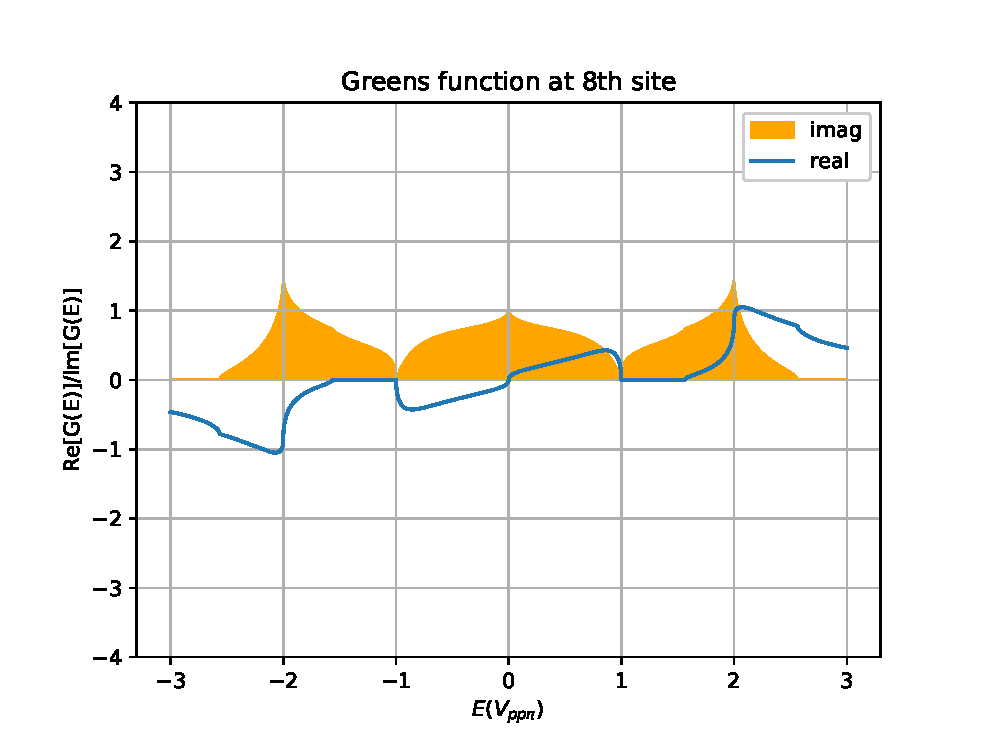
\includegraphics[width=\textwidth]{Figures/BetaimrealTE8.eps}
		\caption{Figure showing a plot of the Green's function at the \nth{8} site}
		\label{4th}
	\end{subfigure}
	~ %add desired spacing between images, e. g. ~, \quad, \qquad, \hfill etc.
	%(or a blank line to force the subfigure onto a new line)
	\begin{subfigure}[b]{0.45\textwidth}
		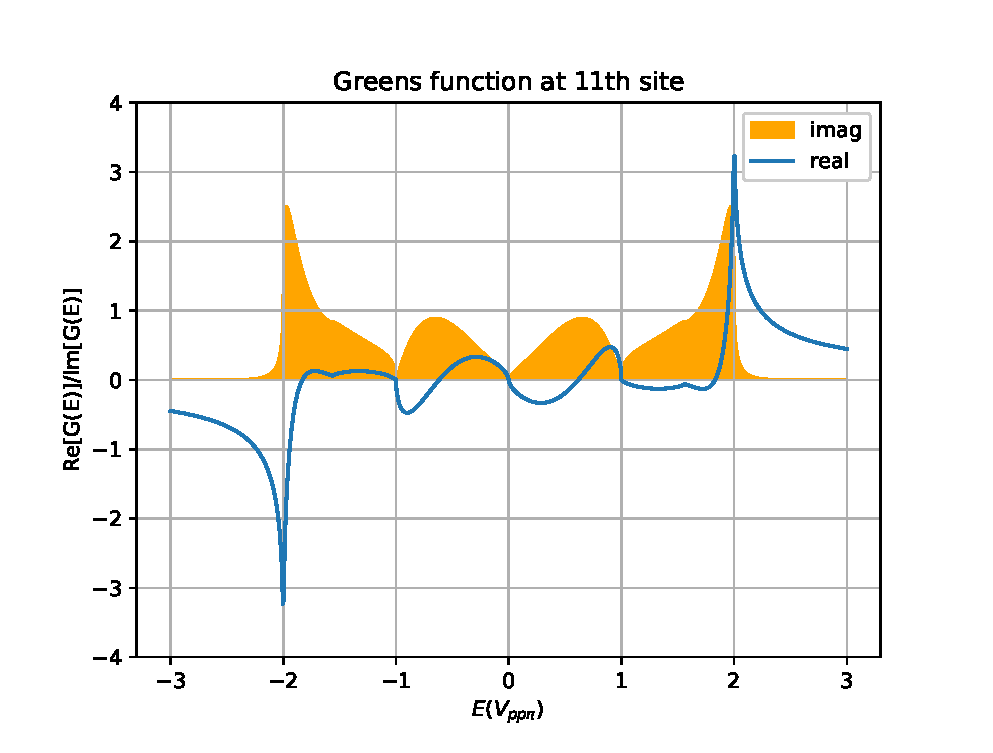
\includegraphics[width=\textwidth]{Figures/BetaimrealTE11.eps}
		\caption{Figure showing a plot of the Green's function at the \nth{11} site}
		\label{7th}
	\end{subfigure}
	\caption{Two plots showing how the Green's function changes as the site is changed. The \nth{8} and \nth{11} sites are corresponding to atoms of those indices (8, 11) in \cref{pointplot}. Note how the LDOS changes (imaginary part) for the different sites.}\label{siteLDOSplot}
\end{figure}
\begin{figure}[h]
	\centering
	\begin{subfigure}[b]{0.3\textwidth}
		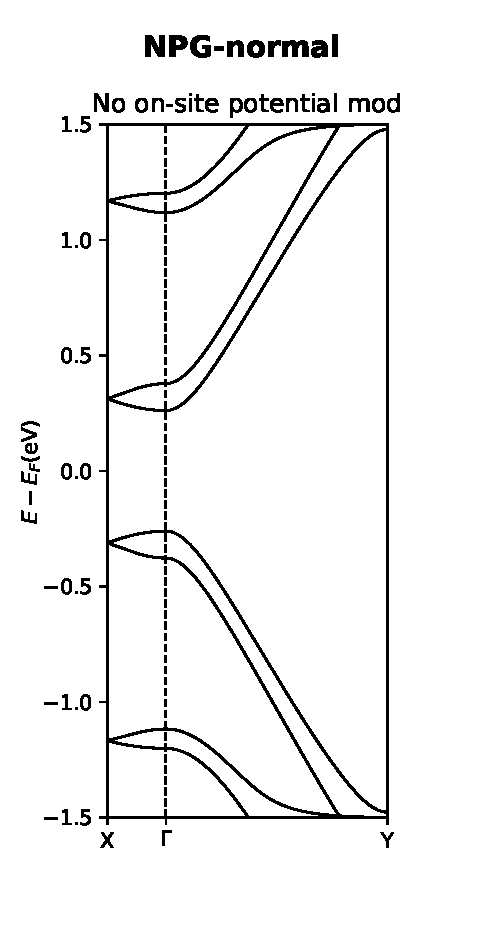
\includegraphics[width=\textwidth]{Figures/FabNPGBS.eps}
		\caption{Normal NPG}
		\label{Fabbs}
	\end{subfigure}
	~ %add desired spacing between images, e. g. ~, \quad, \qquad, \hfill etc.
	%(or a blank line to force the subfigure onto a new line)
	\begin{subfigure}[b]{0.3\textwidth}
		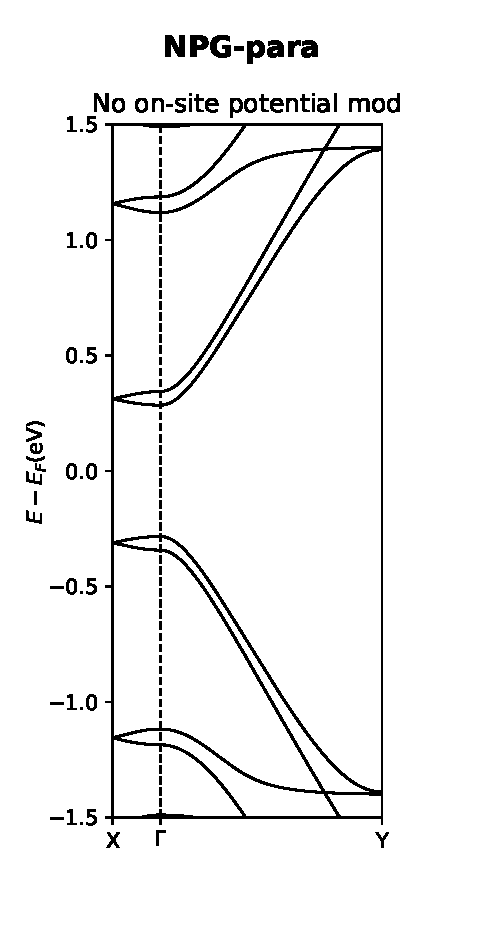
\includegraphics[width=\textwidth]{Figures/paraNPGBS.eps}
		\caption{Para NPG}
		\label{parabs}
	\end{subfigure}
	~ %add desired spacing between images, e. g. ~, \quad, \qquad, \hfill etc.
	%(or a blank line to force the subfigure onto a new line)
	\begin{subfigure}[b]{0.3\textwidth}
		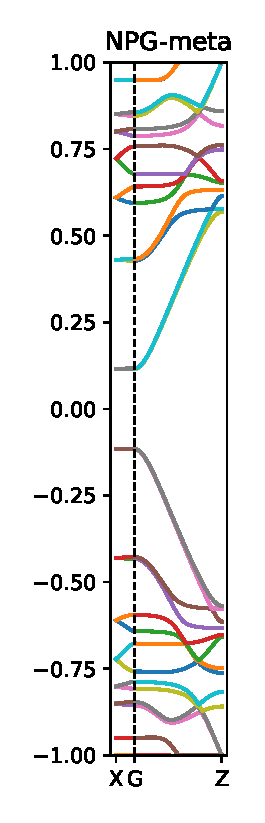
\includegraphics[width=\textwidth]{Figures/metaNPGBS.eps}
		\caption{Meta NPG}
		\label{metabs}
	\end{subfigure}
	\caption{Plot showing band structures in the energy range \SI{-1.5}{\electronvolt} to \SI{1.5}{\electronvolt} for normal, para and meta NPG. The are plotted between symmetry points \(X\) and \(Y\) with respect to the origin \(\Gamma\)}\label{allbands}
\end{figure}

\im{Listings/Functions.py}{245}{252}
\vspace{-1\baselineskip}
\captionof{listing}{Code piece showing how the periodic Hamiltonian, shifted in the transverse direction i created using the given unit vector in the y direction.}{\label{periodichamilcode}}\vspace{\baselineskip}

\im{Listings/Functions.py}{234}{242}
\vspace{-1\baselineskip}
\captionof{listing}{Code piece showing how the transmission per energy point, using equation \cref{transeq}}{\label{transmissioncode}\vspace{\baselineskip}

\newpage
\im{Listings/Functions.py}{237}{245}
\im{Listings/Functions.py}{72}{81}
\im{Listings/Functions.py}{84}{111}
\im{Listings/Functions.py}{198}{234}
% \section{Project overview}
% A Gantt chart is provided on the next page. \textbf{Not Updated.}
% \newpage
% \begin{turnpage}
% \setcounter{myWeekNum}{6}
% \ganttset{%
% 	calendar week text={\myWeek{}}%
% }
% \begin{figure}\vspace{-10mm}
% \begin{ganttchart}[
% 		hgrid,
% 		vgrid={*{6}{draw=none}, dotted},
% 		x unit=.15cm,
% 		%	y unit title=.6cm,
% 		%	y unit chart=.6cm,
% 		inline,
% 		milestone inline label node/.append style={left=5mm},
% 		milestone/.append style={xscale=3},
% 		time slot format=isodate,
% 		time slot format/start date=2019-02-04
% 	]{2019-02-04}{2019-05-31}
% 	\gantttitlecalendar{year, month=shortname, week}\\
% 	\ganttgroup{Report writing}{2019-02-25}{2019-05-31}\\
% 	\ganttgroup[inline = false]{Course 33442}{2019-02-04}{2019-03-31}\\
% 	\ganttbar{Ch. 1 \& 2}{2019-02-04}{2019-02-17}\\
% 	\ganttlinkedbar[link bulge=2]{Ch. 3}{2019-02-18}{2019-02-24}\\
% 	\ganttlinkedbar[link bulge=2,bar inline label node/.style={right=15pt}]{Ch. 4 \& 5}{2019-02-25}{2019-03-03}\\
% 	\ganttgroup[inline = false]{Python code}{2019-03-04}{2019-03-31}\\
% 	\ganttbar{Py TB scripts}{2019-02-18}{2019-03-17}\\
% 	\ganttlinkedbar[link bulge=2, bar inline label node/.style={right=45pt}]{Small NPG systems simulations}{2019-03-10}{2019-03-31}\\
% 	\ganttmilestone{Proof of Concept with Python}{2019-03-31}\\
% 	\ganttgroup[inline = false]{Large scale TB}{2019-04-01}{2019-04-28}\\
% 	\ganttbar[bar inline label node/.style={left=10pt}]{SISL \& TBtrans tutorial}{2019-04-01}{2019-04-05}\\
% 	\ganttlinkedbar[link bulge=2, bar inline label node/.style={right=50pt}]{Setup NPG variations}{2019-04-06}{2019-04-28}\\
% 	\ganttgroup[inline = false]{Generate data}{2019-04-28}{2019-05-31}\\
% 	\ganttmilestone{Hand in report}{2019-05-31}
% \end{ganttchart}
% \end{figure}
% \end{turnpage}
% \clearpage
% \global\pdfpageattr\expandafter{\the\pdfpageattr/Rotate 90}

\end{document}
